%!TEX TS-program = xelatex

% Шаблон документа LaTeX создан в 2018 году
% Алексеем Подчезерцевым
% В качестве исходных использованы шаблоны
% 	Данилом Фёдоровых (danil@fedorovykh.ru) 
%		https://www.writelatex.com/coursera/latex/5.2.2
%	LaTeX-шаблон для русской кандидатской диссертации и её автореферата.
%		https://github.com/AndreyAkinshin/Russian-Phd-LaTeX-Dissertation-Template

\documentclass[a4paper,14pt]{article}


%%% Работа с русским языком
\usepackage[english,russian]{babel}   %% загружает пакет многоязыковой вёрстки
\usepackage{fontspec}      %% подготавливает загрузку шрифтов Open Type, True Type и др.
\defaultfontfeatures{Ligatures={TeX},Renderer=Basic}  %% свойства шрифтов по умолчанию
\setmainfont[Ligatures={TeX,Historic}]{Times New Roman} %% задаёт основной шрифт документа
\setsansfont{Comic Sans MS}                    %% задаёт шрифт без засечек
\setmonofont{Courier New}
\usepackage{indentfirst}
\frenchspacing

\renewcommand{\epsilon}{\ensuremath{\varepsilon}}
\renewcommand{\phi}{\ensuremath{\varphi}}
\renewcommand{\kappa}{\ensuremath{\varkappa}}
\renewcommand{\le}{\ensuremath{\leqslant}}
\renewcommand{\leq}{\ensuremath{\leqslant}}
\renewcommand{\ge}{\ensuremath{\geqslant}}
\renewcommand{\geq}{\ensuremath{\geqslant}}
\renewcommand{\emptyset}{\varnothing}

%%% Дополнительная работа с математикой
\usepackage{amsmath,amsfonts,amssymb,amsthm,mathtools} % AMS
\usepackage{icomma} % "Умная" запятая: $0,2$ --- число, $0, 2$ --- перечисление

%% Номера формул
%\mathtoolsset{showonlyrefs=true} % Показывать номера только у тех формул, на которые есть \eqref{} в тексте.
%\usepackage{leqno} % Нумерация формул слева	

%% Перенос знаков в формулах (по Львовскому)
\newcommand*{\hm}[1]{#1\nobreak\discretionary{}
	{\hbox{$\mathsurround=0pt #1$}}{}}

%%% Работа с картинками
\usepackage{graphicx}  % Для вставки рисунков
\graphicspath{{images/}}  % папки с картинками
\setlength\fboxsep{3pt} % Отступ рамки \fbox{} от рисунка
\setlength\fboxrule{1pt} % Толщина линий рамки \fbox{}
\usepackage{wrapfig} % Обтекание рисунков текстом

%%% Работа с таблицами
\usepackage{array,tabularx,tabulary,booktabs} % Дополнительная работа с таблицами
\usepackage{longtable}  % Длинные таблицы
\usepackage{multirow} % Слияние строк в таблице
\usepackage{float}% http://ctan.org/pkg/float

%%% Программирование
\usepackage{etoolbox} % логические операторы


%%% Страница
\usepackage{extsizes} % Возможность сделать 14-й шрифт
\usepackage{geometry} % Простой способ задавать поля
\geometry{top=20mm}
\geometry{bottom=20mm}
\geometry{left=20mm}
\geometry{right=10mm}
%
%\usepackage{fancyhdr} % Колонтитулы
% 	\pagestyle{fancy}
%\renewcommand{\headrulewidth}{0pt}  % Толщина линейки, отчеркивающей верхний колонтитул
% 	\lfoot{Нижний левый}
% 	\rfoot{Нижний правый}
% 	\rhead{Верхний правый}
% 	\chead{Верхний в центре}
% 	\lhead{Верхний левый}
%	\cfoot{Нижний в центре} % По умолчанию здесь номер страницы

\usepackage{setspace} % Интерлиньяж
\onehalfspacing % Интерлиньяж 1.5
%\doublespacing % Интерлиньяж 2
%\singlespacing % Интерлиньяж 1

\usepackage{lastpage} % Узнать, сколько всего страниц в документе.

\usepackage{soul} % Модификаторы начертания

\usepackage{hyperref}
\usepackage[usenames,dvipsnames,svgnames,table,rgb]{xcolor}
\hypersetup{				% Гиперссылки
	unicode=true,           % русские буквы в раздела PDF
	pdftitle={Заголовок},   % Заголовок
	pdfauthor={Автор},      % Автор
	pdfsubject={Тема},      % Тема
	pdfcreator={Создатель}, % Создатель
	pdfproducer={Производитель}, % Производитель
	pdfkeywords={keyword1} {key2} {key3}, % Ключевые слова
	colorlinks=true,       	% false: ссылки в рамках; true: цветные ссылки
	linkcolor=black,          % внутренние ссылки
	citecolor=black,        % на библиографию
	filecolor=magenta,      % на файлы
	urlcolor=black           % на URL
}
\makeatletter 
\def\@biblabel#1{#1. } 
\makeatother
\usepackage{cite} % Работа с библиографией
%\usepackage[superscript]{cite} % Ссылки в верхних индексах
%\usepackage[nocompress]{cite} % 
\usepackage{csquotes} % Еще инструменты для ссылок

\usepackage{multicol} % Несколько колонок

\usepackage{tikz} % Работа с графикой
\usepackage{pgfplots}
\usepackage{pgfplotstable}

% ГОСТ заголовки
\usepackage[font=small]{caption}
%\captionsetup[table]{justification=centering, labelsep = newline} % Таблицы по правобу краю
%\captionsetup[figure]{justification=centering} % Картинки по центру


\newcommand{\tablecaption}[1]{\addtocounter{table}{1}\small \begin{flushright}\tablename \ \thetable\end{flushright}%	
\begin{center}#1\end{center}}

\newcommand{\imref}[1]{рис.~\ref{#1}}

\usepackage{multirow}
\usepackage{spreadtab}
\newcolumntype{K}[1]{@{}>{\centering\arraybackslash}p{#1cm}@{}}


\usepackage{xparse}
\usepackage{fancyvrb}

\RecustomVerbatimCommand{\VerbatimInput}{VerbatimInput}
{
	fontsize=\footnotesize    
}

\usepackage{tocloft}
\renewcommand{\cftsecleader}{\cftdotfill{\cftdotsep}}
\begin{document} % конец преамбулы, начало документа
	\begin{titlepage}
	\begin{center}
 		ФЕДЕРАЛЬНОЕ  ГОСУДАРСТВЕННОЕ АВТОНОМНОЕ \\
		ОБРАЗОВАТЕЛЬНОЕ УЧРЕЖДЕНИЕ ВЫСШЕГО ОБРАЗОВАНИЯ\\
		«НАЦИОНАЛЬНЫЙ ИССЛЕДОВАТЕЛЬСКИЙ УНИВЕРСИТЕТ\\
		«ВЫСШАЯ ШКОЛА ЭКОНОМИКИ»
	\end{center}
	
	\begin{center}
		\textbf{Московский институт электроники и математики}
		
		\textbf{им. А.Н.Тихонова НИУ ВШЭ}
		
		\vspace{2ex}
		
		\textbf{Департамент компьютерной инженерии}
	\end{center}
	\vspace{1ex}	
	
	\begin{center}
		Курс «Системное проектирование цифровых устройств»
	\end{center}	
	
	
	\begin{center}
	\textbf{ОТЧЕТ\\
		ПО ЛАБОРАТОРНОЙ РАБОТЕ №5
	}
	\end{center}	

	\begin{center}
		Тема работы: «Обработка звука на ПЛИС»
	\end{center}

	\vspace{2ex}

	\begin{flushright}
		\textbf{Выполнили:}
		
		\vspace{2ex}
		
		Студенты группы БИВ174
		
		Бригада №5
		
		\vspace{2ex}
		
		Подчезерцев Алексей Евгеньевич
		
		Солодянкин Андрей Александрович
		\vspace{2ex}
		
		\textbf{Принял:}
		
		асс. МИЭМ НИУ ВШЭ
		
		Американов А.А.
		
	\end{flushright}

	\vfill
	\begin{center}
		Москва \the\year \, г.
	\end{center}
	
\end{titlepage}
\addtocounter{page}{1}
	\tableofcontents
	\pagebreak
	\section{Задание}
	
	\begin{enumerate}
		\item Изучить разделы 6.2, 6.3, 6.4, 6.7 и приложение В книги H\&H.
		Добавить в микропроцессор в соответствии со своим вариантом	поддержку следующих команд: j, xori, sllv, nor.
		
		\item Разработать программу, продемонстрировать на модели и прототипе правильность их работы.
		Разработать в соответствии со своим вариантом программу, продемонстрировать на модели и прототипе правильность ее работы.
		Добавить ее в проект микропроцессора; добавить в папку с программой файл описания.
		Использовать только те команды, которые есть в процессоре.
		
		6) Найти сумму геометрической прогрессии (количество членов прогрессии = ваш
		вариант \% 30 + 3, знаменатель прогрессии = ваш вариант \% 10 + 1)
		
		\item Перейти в ветку проекта schoolMIPS 01\_mmio.
		Скачать новую версию процессора и выполнить на вашей плате (или DE10-Lite)
		программы 00\_counter, 01\_fibonacci, 02\_sqrt. Убедиться, что они работают также.
		Выполнить одну из программ (по вариантам):
		
		2) 04\_gpio
	\end{enumerate}

	%{\small \VerbatimInput{../03_syn_pow_5_single_cycle_always/pow_5_single_cycle_always.v}}
	
	\section{Выполнение работы}
	
	\subsection{Моделирование счетчика}
	
	Ассемблерный код счетчика представлен на листинге ниже.
	
	{\small \VerbatimInput{../program/00_counter/main.S}}
	
	Моделирование программы проводилось в среде Icarus Verilog.
	
	Ниже приведена часть логов из выполнения программы:
	
	{\small \VerbatimInput{./logs/00_logs.txt}}
	
	Вейвформа при моделировании программы (рис. \ref{fig:00wvf}).
	
	\begin{figure}[H]
		\centering
		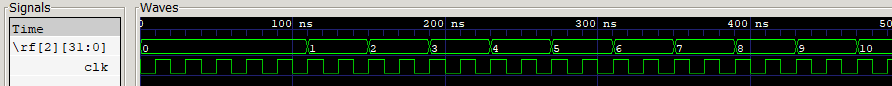
\includegraphics[width=0.95\linewidth]{images/00_wvf}
		\caption{Вейвформа для программы счетчика}
		\label{fig:00wvf}
	\end{figure}

	Можно заметить, что значение интересующего нас регистра постепенно увеличивается на 1, результат помещается в регистр v0.
	
	
	\subsection{Моделирование последовательности Фибоначчи}
	
	Ассемблерный код функции для подсчета значений последовательности Фибоначчи представлен на листинге ниже.
	
	{\small \VerbatimInput{../program/01_fibonacci/main.S}}
	
	Моделирование программы проводилось в среде Icarus Verilog.
	
	Ниже приведена часть логов из выполнения программы:
	
	{\small \VerbatimInput{./logs/01_logs.txt}}
	
	Вейвформа при моделировании программы (рис. \ref{fig:01wvf}).
	
	\begin{figure}[H]
		\centering
		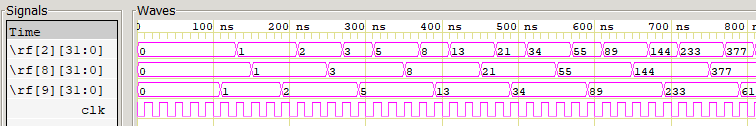
\includegraphics[width=0.95\linewidth]{images/01_wvf}
		\caption{Вейвформа для последовательности Фибоначчи}
		\label{fig:01wvf}
	\end{figure}

	В регистре v0 помещается текущее значение последовательности Фиббоначи.
	

	\subsection{Моделирование извлечения квадратного корня}
	
	Ассемблерный код функции для вычисления квадратного корня представлен на листинге ниже.
	
	{\small \VerbatimInput{../program/02_sqrt/main.S}}
	
	Моделирование программы проводилось в среде Icarus Verilog.
	
	Лог выполнения программы:
	
	{\small \VerbatimInput{./logs/02_sqrt_logs.txt}}
	
	Вейвформа при моделировании программы (рис. \ref{fig:02wvf}).
	
	\begin{figure}[H]
		\centering
		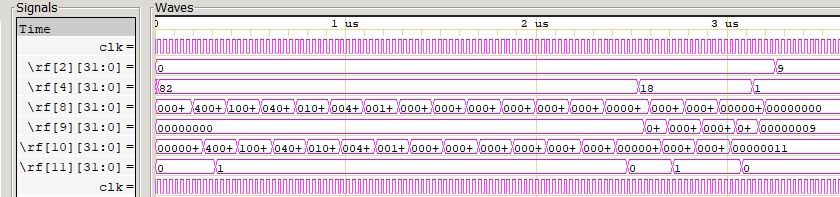
\includegraphics[width=0.95\linewidth]{images/02_wvf}
		\caption{Вейвформа для программы извлечения квадратного корня}
		\label{fig:02wvf}
	\end{figure}

	Результат вычисления программы помещается регистр v0.
	
	
	\section{Самостоятельная работа}
	
	\subsection{Добавление новых команд}
	
	В соответствии с заданием необходимо добавить команды: j, xori, sllv, nor.
	
	Команда безусловного перехода j записывает новое значение в счётчик команд \cite{Harris}.
	Для реализации данной команды необходимо добавить новый выход у Control unit, который будет отвечать за безусловный переход.
	В случае установки данного флага будет изменено значение счетчика команд (PC).
	Адрес перехода получается из второй части команды j.
	
	Для реализации остальных команд необходимо расширить возможности ALU: добавить операции xor, sll, nor.
	После этого добавляются строки в мультиплексор, которые отвечают за распознавание команд.
	Команда xori является операцией I-типа и работает с константой, остальные операции R-типа и работают с регистрами.
	
	Для тестирования кода была написана небольшая программа на ассемблере:
		
	{\small \VerbatimInput{../program/98_commands_visualization/main.S}}
	
	Моделирование программы проводилось в среде Icarus Verilog.
	
	Лог выполнения программы:
	
	{\small \VerbatimInput{./logs/98_commands_visualization.txt}}
	
	\subsection{Разработка программы нахождения суммы геометрической прогрессии}
	
	Ассемблерный код функции для вычисления суммы геометрической прогрессии представлен на листинге ниже.
	
	{\small \VerbatimInput{../program/99_geometric_progression/main.S}}
	
	После метки старт происходит инициализация значений в соответствии с вариантом.
	Далее выполняются команды внутри метки for\_loop, где на каждом цикле вычисляется новое значение геометрической прогрессии.
	Умножение реализовано в виде функции в метке multiplyer.
	Когда вычисленно нужное число членов геометрической прогрессии, цикл for\_loop завершается и выполняется код под меткой end.
	В метке end вычисленная сумма перемещается в регистр v0.
	
	Моделирование программы проводилось в среде Icarus Verilog.
	
	Лог выполнения программы:
	
	{\small \VerbatimInput{./logs/99_logs.txt}}
	
	Вейвформа при моделировании программы (рис. \ref{fig:99wvf}).
	
	\begin{figure}[H]
		\centering
		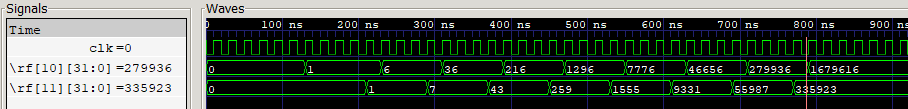
\includegraphics[width=0.95\linewidth]{images/99_wvf}
		\caption{Вейвформа для суммы геометрической прогрессии}
		\label{fig:99wvf}
	\end{figure}

	Результаты из программы Mars совпадают c результатами из моделирования (рис. \ref{fig:99mars}).

	\begin{figure}[H]
		\centering
		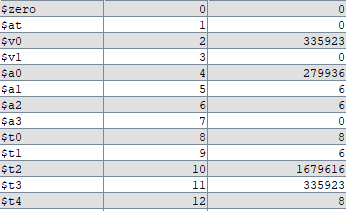
\includegraphics[width=0.5\linewidth]{images/99_mars}
		\caption{Результаты моделирования в программе Mars}
		\label{fig:99mars}
	\end{figure}

	\subsection{Моделирование программ на процессоре из ветки 01\_mmio}
	
	Было произведено моделирование программ  00\_counter, 01\_fibonacci, 02\_sqrt, все по-прежнему работают, но никаких изменений в логах или вейвформах нет.
	
	Моделирование 
	
	\section{Выводы по работе}
	
	В ходе работы получен опыт проектирования схем в программе Quartus с помощью языка Verilog.
	Полученное устройство было протестировано с помощью бенчтестов в программе Quartus Simulation Waveform editor.
	В процессе работы были смоделированы устройства для конвейерной обработки данных и изучены различные способы моделирования.
	В процессе был получен опыт работы с платой DE10-Lite, на которой проверялась работоспособность полученного устройства.
	
	\newpage 
	\renewcommand{\refname}{{\normalsize Список использованных источников}} 
	\centering 
	\begin{thebibliography}{9} 
		\addcontentsline{toc}{section}{\refname} 
		\bibitem{Harris} Хэррис Д. М., Хэррис С. Л. Цифровая схемотехника и архитектура компьютера. – 2015.
	\end{thebibliography}
	
\end{document} % конец документа
